\input{preamble.tex}
% dove sono le immagini'
\graphicspath{ {./figures/} }

% ACRONIMI
% \newacronym{label}{acronimo}{acronimo esteso}
\newacronym{sts}{STS}{Space Transportation System}
\newacronym{iss}{ISS}{International Space Station}
\newacronym{nasa}{NASA}{National Aeronautics and Space Administration}
\newacronym{ssme}{SSME}{Space Shuttle Main Engine}
\newacronym{srb}{SRB}{Solid Rocket Boosters}
\newacronym{lh2}{$LH_2$}{liquid hydrogen}
\newacronym{lox}{$LO_2$}{liquid oxygen}
\newacronym{lch4}{$LCH_4$}{liquid methane}
\newacronym{lptp}{LPTP}{low pressure turbopump}
\newacronym{hptp}{HPTP}{high pressure turbopump}
\newacronym{et}{ET}{external tank}

\title{Space Shuttle Main Engine: fuel and tank analysis}
\begin{document}
    \maketitle
    \tableofcontents
    \newpage
    \printglossary[type=\acronymtype]
    \newpage
% --- SCRIVERE QUI ---
    \section{Introduction} \label{intro}
    Space exploration represents one of the most fascinating and complex frontiers of contemporary science and technology. 
	At the heart of this field is the \acrfull{sts}, commonly known as the Space Shuttle launch system, which played a fundamental role in the development of human capabilities to explore and utilize space.
	Operated by \acrshort{nasa} from 1981 to 2011, the Space Shuttle was the first reusable space transportation system, an innovative orbital vehicle that combined the characteristics of a rocket and an airplane.
The Space Shuttle program enabled numerous scientific and technical missions, including the launch of satellites, the construction, maintenance of the \acrfull{iss} and a variety of scientific experiments in orbit.
This vehicle allowed astronauts and payloads to be transported into space and returned to Earth, marking a turning point in the history of astronautics.


The launch system consists of three RS-25 (\acrshort{ssme}) and two additional \acrfull{srb}. The \acrfull{ssme} was one of the most advanced and crucial technological elements of the \acrshort{sts}. The \acrshort{ssme}s were the primary rocket engines, propelled by \acrfull{lh2} and \acrfull{lox}, providing the necessary thrust for the Shuttle's liftoff and initial ascent to low Earth orbit. These engines were known for their efficiency and reliability, being able to operate under extreme conditions and be reused for multiple launches.

    %The Space shuttle propulsion system consists of three space shuttle main engines (SSME) which draw liquid oxigen ($ LO_2 $) and liquid hydrogen ($ LH_2 $) from the external tank (ET).On the sides of the ET two solid rocket boosters are attached.To control the attitude of the orbiter, once it has reached space, two orbital manouvering system (OMS) engines and 44 reaction control systems (RCS) thrusters are used.The following is an analysis of the SSME's thermodynamic cycle and how the propulsive properties change when another fuel is used instead of $ LH_2 $. 

The purpose of this report is to initially size the real \acrfull{ssme} and then, based on the total impulse and burning time of this engine, to resize the engine while changing the fuel from \acrlong{lh2} to \acrfull{lch4}. 
This analysis anticipates a simplification of the system components and a reduction in the mass of the \acrfull{et} given that methane has a much higher density than hydrogen. Additionally, the storage temperature of methane is very similar to that of oxygen, which could help avoid issues related to thermal exchange between the fuel and oxidizer tanks.
The path followed in this report involved taking upstream and downstream pressures of each component, the inlet temperatures to the various components, and the mass flow rates of the fuel and oxidizer. Using these parameters, the turbopumps, injectors, combustion chamber, nozzle, and \acrlong{et} were appropriately sized through MATLAB. For the engine's performance analysis, NASA's CEA software was utilized. Subsequently, by observing these performances and using the burning time, O/F ratio, total engine impulse, and combustion chamber pressure as starting points, the engine was resized for the new fuel \acrshort{lch4} by working backward from these parameters.
\section{Staged combustion cycle description}
The Stage Combustion Cycle used in the Space Shuttle Main Engine (SSME) is a highly efficient and intricate system specifically designed for maximum performance.
In the SSME, this cycle involves the partial combustion of both liquid hydrogen (fuel) and liquid oxygen (oxidizer) in separate preburners. 
The preburners produce hot, high-pressure, fuel-rich gases that drive the engine's turbopumps, which in turn feed the remaining propellants into the main combustion chamber at extremely high pressures.
What sets the SSME apart is its use of a closed-cycle stage combustion process, where all the exhaust gases from the preburners are directed into the main combustion chamber, ensuring that no energy is wasted.
This results in very high efficiency, with the SSME achieving one of the highest specific impulses of any rocket engine.
The high pressures and temperatures involved in this cycle make it extremely complex, but they also enable the SSME to deliver the power needed for the Space Shuttle's demanding missions.




As stated in \cref{intro} the original \acrshort{ssme} cycle uses \acrlong{lh2} and \acrlong{lox}. After being withdrawn from the \acrfull{et} both the fuel and the oxidizer go through a \acrfull{lptp}, a \acrfull{hptp} and a preburner before meeting in the combustion chamber. What follows is an analysis of every turbomachine of the cycle.
\begin{figure}
	\centering
 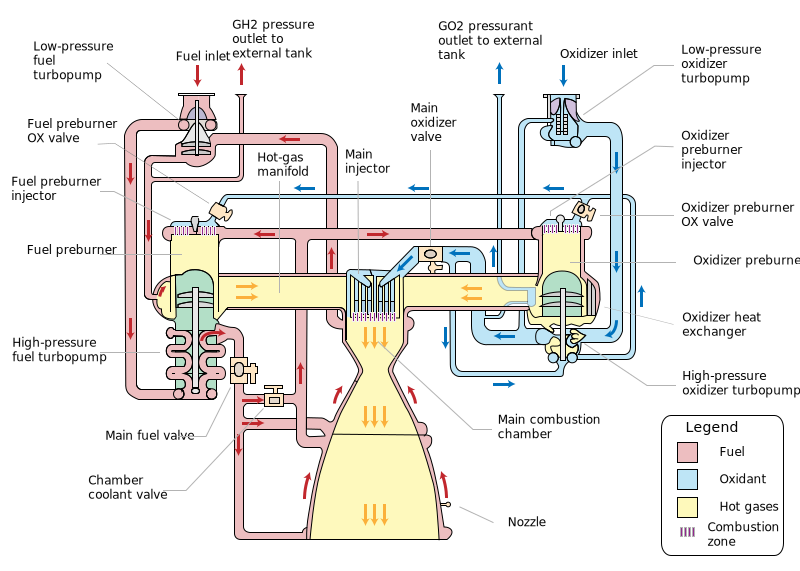
\includegraphics[width=.75\textwidth]{ssme_ciclo}
	\caption{A functional diagram showing the flow of propellant through an RS-25 engine.}
	\label{fig:ssme_cycle}
\end{figure}
\Cref{fig:ssme_cycle} is missing some components, such as the pogo oscillation suppression system accumulator, mounted before the oxidizer \acrshort{hptp}. However this goes beyond the scope of our analysis and will be disregarded.
 \end{document}
